\begin{bibunit}
\thispagestyle{plain}

% Define commands used in the paper
\newcommand{\codeword}[1]{\texttt{\detokenize{#1}}}
\newcommand{\quotes}[1]{``#1''}

% Ensure proper figure placement
\setcounter{topnumber}{2}
\setcounter{bottomnumber}{2}
\setcounter{totalnumber}{4}
\renewcommand{\topfraction}{0.85}
\renewcommand{\bottomfraction}{0.65}
\renewcommand{\textfraction}{0.15}
\renewcommand{\floatpagefraction}{0.7}



\section*{Abstract}
    Automation systems within nuclear laboratories are intended to work under harsh operating conditions. SPES (Selective Production of Exotic Species) is a nuclear research facility currently under construction by INFN (Istituto Nazionale di Fisica Nucleare), dedicated to the production and study of Radioactive Ion Beams (RIBs). Isotopes are produced within the Target Ion Source (TIS) unit, a vacuum vessel that must be replaced on a regular basis. The highly radioactive environment necessitates the deployment of a set of automated systems dedicated to the unit's remote management. To meet high-level security standards, the design of such instrumentation and control systems must include extensive verification. Based on specific safety requirements, model checking can be used to assess the systems' correctness. This paper describes how to employ an integrated tool-chain to design, simulate, formally verify, and deploy the control software for the Horizontal Handling Machine, a safety-critical remote handling system in operation at SPES. The IEC 61499 standard's adoption led to a redesign of the control logic. Following a preliminary online simulation, the closed-loop system has been formally verified using the NuSMV symbolic model checker, with the help of the FB2SMV converter. Additionally, the FBME tool was used for automating verification and analyzing counterexamples.

\section{Introduction}
\label{sec:introduction}
Automation systems in nuclear laboratories must comply with strict safety requirements to avoid any potential risk to personnel or equipment.
The critical operating environment generally discourages innovation in the design of control software, leading to an old-fashioned approach still today in the Industry 4.0 era. However, the introduction of distributed control systems based on modern standards would be advantageous for operational and safety challenges. This paradigm shift will lead to the development of smarter systems based on flexible and reconfigurable automation architectures. In this context, the evolution from applications based on \mbox{IEC 61131-3} \cite{iec61131-3} towards IEC 61499 \cite{iec61499, zoitl2014} solutions would provide key tools to face the design and verification challenges typical of complex distributed control systems. 
The main advantages of this migration include:

\begin{itemize}
    \item Flexible, reconfigurable, and scalable architecture.
    \item Modular design, standardized Function Blocks.
    \item Simulations, offline and online verification. 
    \item Formal model checking techniques.
\end{itemize}

% Figure: HHM
\begin{figure}[h!]
    \centering
    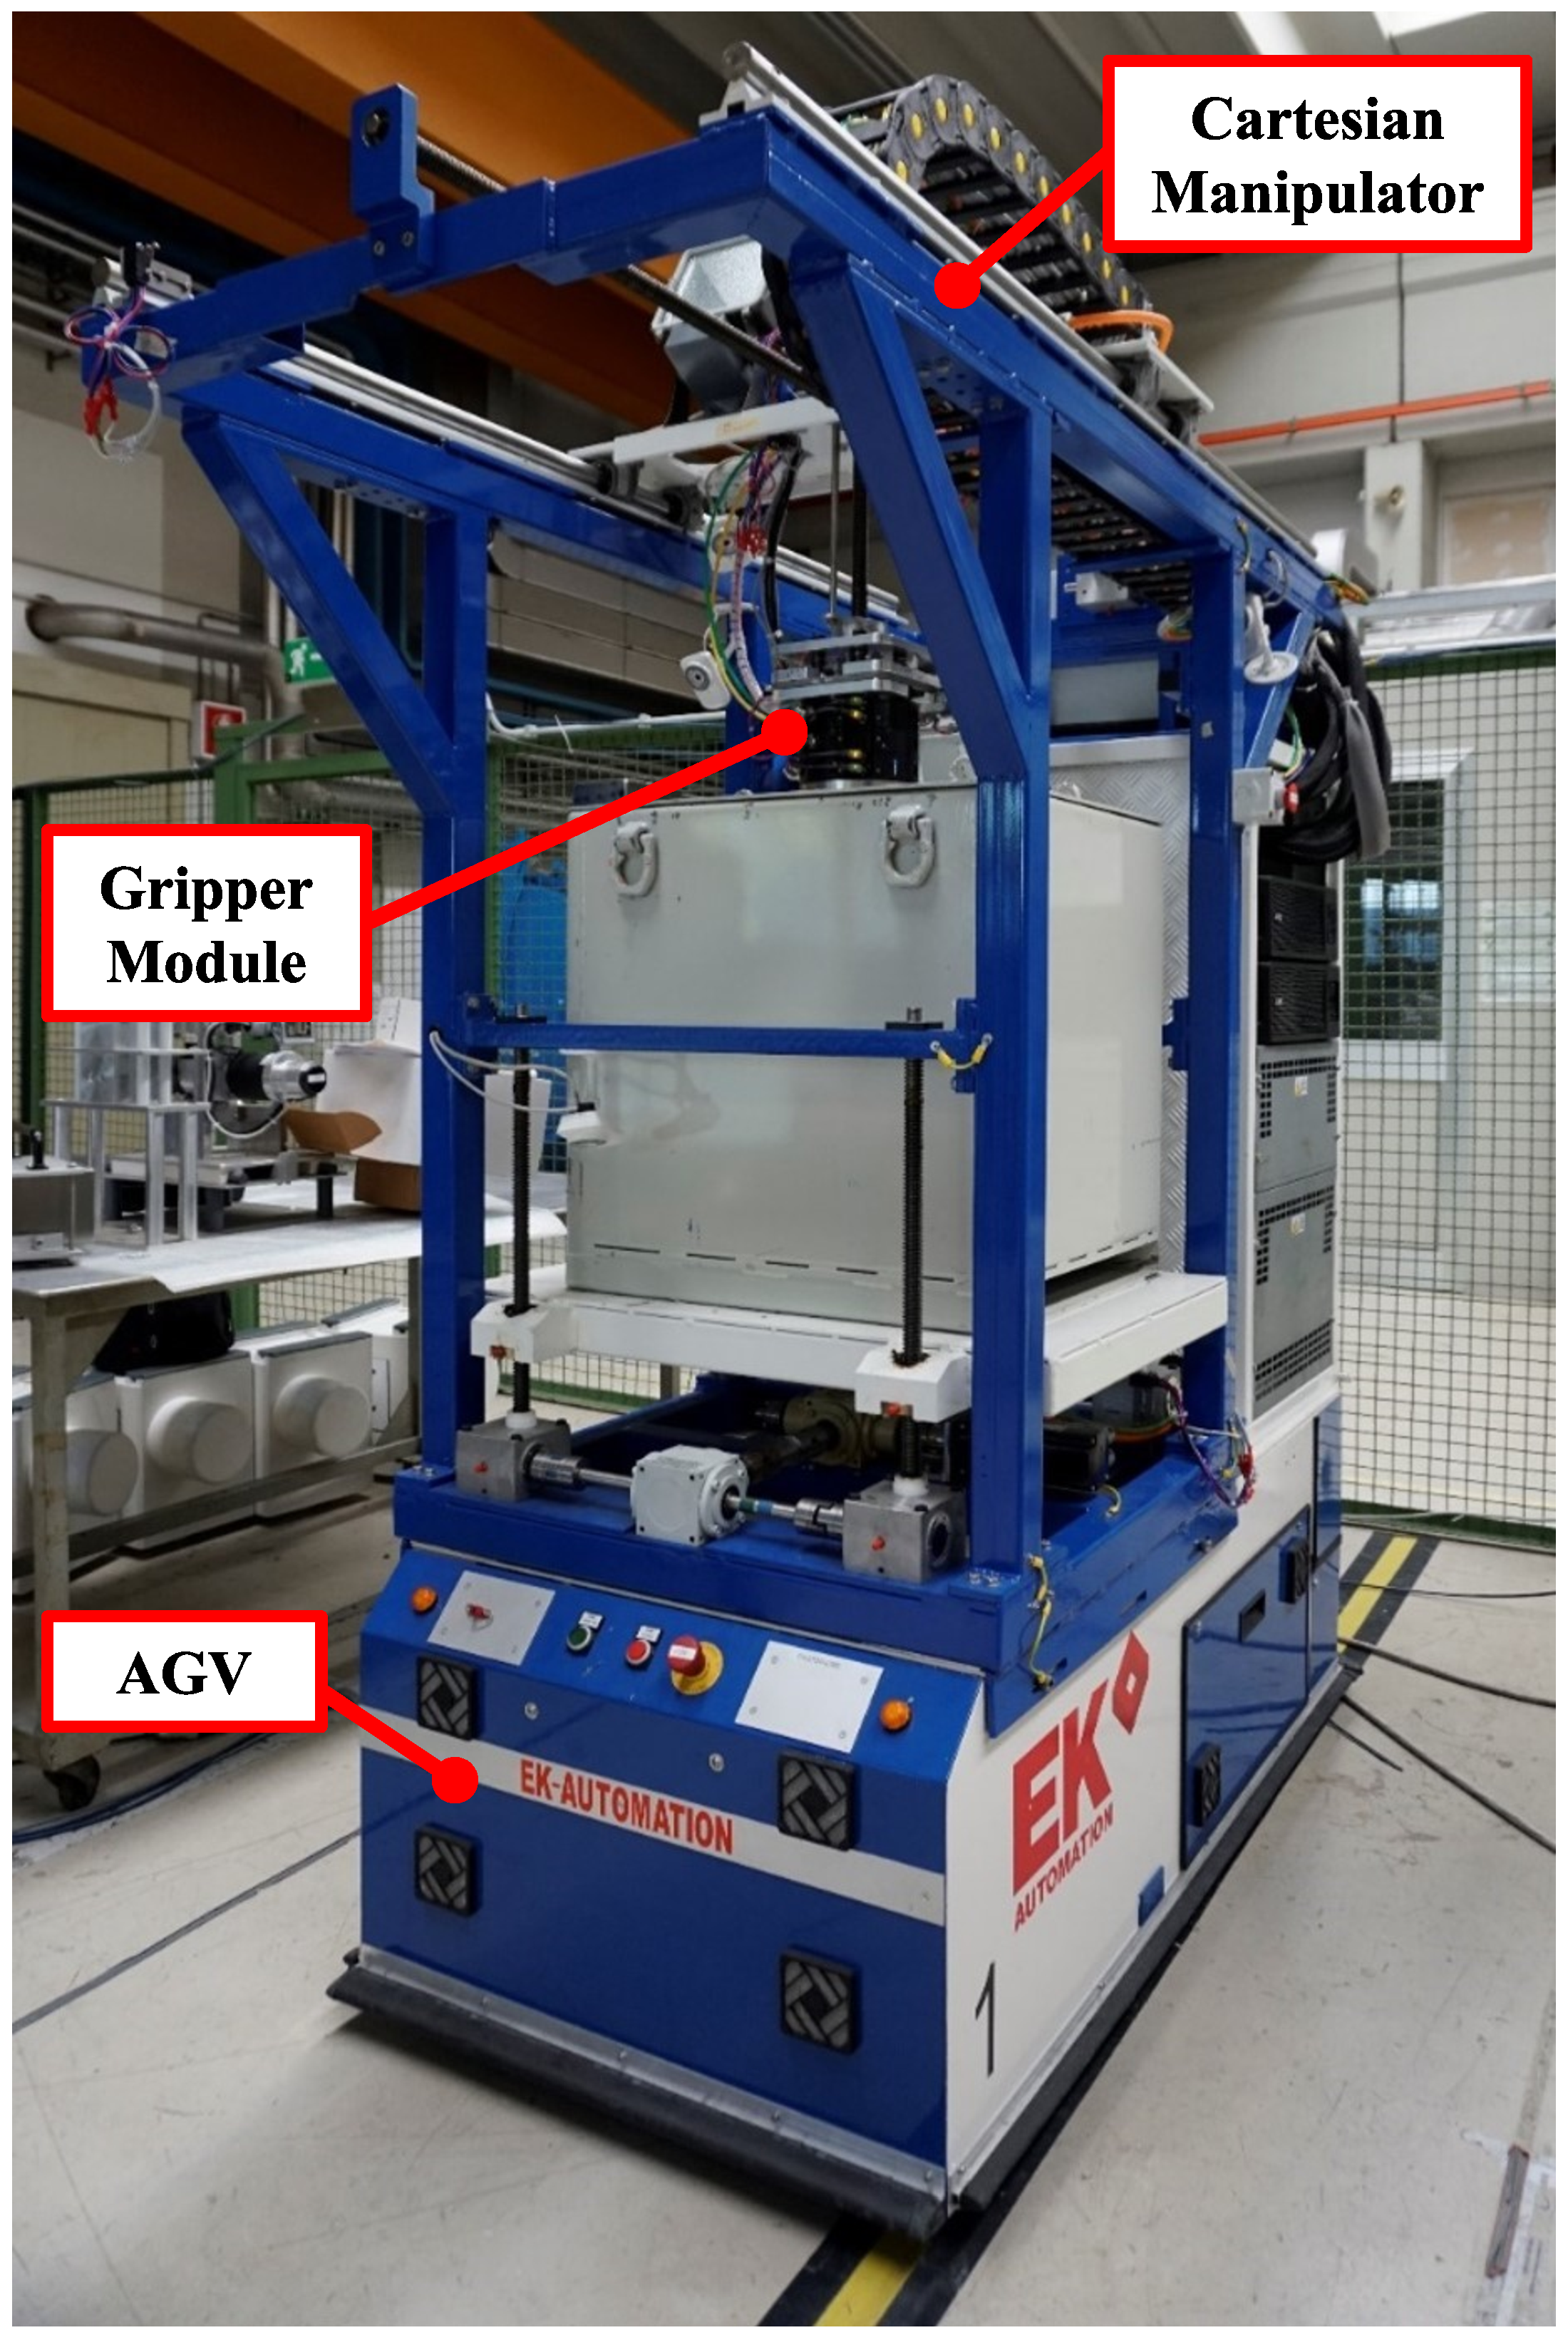
\includegraphics[width=0.8\columnwidth]{MX_Papers/Paper4/pictures/lilli01.eps}
    \caption{The Horizontal Handling Machine (HHM) is the primary remote handling vehicle in operation at the SPES facility.} 
    \label{fig:hhm}
\end{figure}

\noindent The SPES (Selective Production of Exotic Species) facility \cite{Marchietal.2020} can be considered an attractive use case to demonstrate the advantages of implementing safety-critical control systems based on IEC 61499. INFN (Istituto Nazionale di Fisica Nucleare) is currently developing an experimental plant at Legnaro National Laboratories (LNL) for multidisciplinary research on Radioactive Ion Beams (RIBs) produced through the ISOL (Isotope Separation On-Line) technique \cite{Andrighetto2018}. Isotopes are generated, as fission reaction products, from the collision of a high-energy proton beam (40 MeV, 200 $\mu$A) with a multi-foil uranium carbide target \cite{Andrighetto2019} consisting of seven UCx disks \cite{Corradetti2021}. The Target Ion Source (TIS) unit \cite{Monetti2015} is identified as the core of the process. Here the isotopes are produced and extracted for further studies in the field of nuclear physics and for medical applications. Unfortunately, aging of target and source materials requires regular replacement of the TIS unit to maintain high efficiency. This is difficult in view of the specific operational conditions. Indeed, the highly radioactive environment precludes any human operation.
For this reason, the management of the TIS unit is entrusted to a remote handling framework \cite{lilli2023}, conceived to fulfill its specific life cycle. The safe operation and reliability of mobile robots operating in complex scientific facilities are essential features that need to be assessed \cite{khan2014}. In the SPES case, the automated systems involved in the replacement procedure face an intense radiation field generated by various contributions, such as the TIS unit \cite{Monetti2015}, the residual Front-End activation \cite{Donzella2020}, and the isotopes deposition along the RIB line \cite{Centofante2021Study}. 
Operational safety is the outcome of an integrated strategy that combines the formal verification of control software with the deployment of inherently safe design principles to the hardware.
In our work, we focused on the most critical remote handling task: the automated removal of a radioactive TIS unit from the SPES Front-End.
The main objectives of the study are to demonstrate the benefits of the migration of \mbox{IEC 61131-based} software to an IEC 61499 architecture and to implement offline and online software verification techniques. This contribution describes the development of flexible and reconfigurable control software based on IEC 61499, along with its formal verification through an integrated tool-chain, for a safety-critical remote handling system: the Horizontal Handling Machine (HHM) depicted in Fig. \ref{fig:hhm}. 
The provided implementation demonstrates how to incorporate modular Non-Deterministic Transitions (NDTs) in formal verification to improve the mode's realism while limiting complexity. 
The paper is structured as follows: Section \ref{sec:problem_statement} discusses the related works and the problem statement. Section \ref{sec:case_study} explains the design and formal verification approach adopted for a radioactive material remote handling system. Sections \ref{sec:simulation} and \ref{sec:formal_verification} describe the approach used to perform online simulations and formal verification, respectively. Section \ref{sec:results} presents the main results of the work, whereas Section \ref{sec:conclusion} concludes the article and outlines future goals.

\section{Related works and problem statement}
\label{sec:problem_statement}
Designing control systems for industrial applications, particularly those involving nuclear-based materials, is of utmost importance. It is essential to adopt an approach that offers a flexible, portable, reconfigurable, and scalable architecture. 
In this context, the use of design patterns within the field of industrial Cyber-Physical Systems (iCPS) employing the IEC 61499 standard emerges as a favorable strategy for designing such systems \cite{dai2017discrete, patil2018}. 
These design patterns, originating from experienced system designers, hold significant value in the field of software engineering \cite{gamma1995design}.

\subsection{IEC 61499: A model-driven approach to build complex control systems}
IEC 61499 \cite{iec61499} is a standardized framework employed in the field of industrial automation for the modeling of distributed control systems \cite{drozdov2021}. The language's flexibility greatly contributed to its popularity for this type of projects. 
The use of advanced design patterns is crucial during the development of applications, which are defined as platform-independent models composed of modular components, in order to properly exploit this potential, achieving a high level of reusability, and ensuring greater reconfigurability of the underlying systems \cite{sonnleithner2021iec}.
Christensen et al. \cite{christensen2000design} introduced a model-driven approach for distributed control systems, employing the Model-View-Control (MVC) design pattern \cite{Model-view-controller} within the context of IEC 61499 systems. 
The existing body of literature has extensively investigated a variety of model-driven software design and engineering approaches that can be employed for the development of control systems, with a particular emphasis on their application to iCPS \cite{sandeep2018}.
In \cite{bonfe2013design}, the authors examine the packaging industry practices and present design patterns specifically tailored for model-driven software design and implementation. Moreover, similar design patterns are proposed in \cite{cengic2006framework, vyatkin2005architecture, hametner2010automation}.

Safety of control software is an additional factor that becomes crucial in specific applications, such as laboratories dealing with nuclear-based materials.
In these contexts, comprehensive testing is imperative to mitigate the risk of potentially catastrophic issues arising from even minor errors. 
The verification challenge of IEC 61499 has been acknowledged since the early stages of the standard's development and evaluation \cite{vyatkin1999modeling,hanisch2009one}. To achieve the most thorough verification, closed-loop modeling has been suggested, necessitating the inclusion of plant modeling \cite{vyatkin2008closed}. The implementation of a model-driven approach facilitates simulation-in-the-loop \cite{hegny2010iec, yang2012transformation}, enabling thorough testing and identification of system errors. 

During the design process, simulation plays a crucial role in assessing the overall behavior of the control system, ensuring its compliance with expected outcomes and assisting in the process of virtual commissioning \cite{galkin2023automatic}. However, despite being advantageous in identifying flaws, this tool does not provide a guarantee of system reliability. 
Formal verification techniques have thus been proposed, as a promising approach to automatically verify the correctness and safety of automation systems.
Specifically, the model checking integration in closed-loop verification \cite{xavier2023formal} assists in the identification of design weaknesses in the model through the use of counterexamples. The closed-loop architecture, encompassing both the controller and the plant, depicts the overall behavior of the system. This design approach works successfully for both simulation and formal modeling applications \cite{sinha2019survey}. 

% Figure: workflow
\begin{figure*}
    \centering
    \includegraphics[width=\textwidth]{MX_Papers/Paper4/pictures/lilli02.pdf}
    \caption{Proposed workflow for the validation of safety-critical automation systems.} 
    \label{fig:workflow}
\end{figure*}

\subsection{Formal Verification Techniques for  Modular Industrial Control Systems: Challenges and Strategies}

Model checking includes formal verification methods that are used as trustworthy tools to grant the correctness of Instrumentation and Control (I\&C) systems \cite{clarke1999, schneider2004, baier2008}.
These techniques have been employed in a wide range of disciplines, including avionics \cite{gelman2013, wang2019}, automotive \cite{todorov2018, kim2015, Filipovikj2016}, and Nuclear Power Plants (NPP) \cite{pakonen2021, Jee2010, nemeth2009, adiego2015}.
Despite their remarkable benefits for the validation of complex automation control logics, the computing requirements of model checking techniques may frequently represent a bottleneck in their use \cite{Buzhinsky2020}. Several approaches have thus been proposed to reduce their computational complexity \cite{Cimatti2012, Biere2003, burch1992}.
Furthermore, special care should be taken to guarantee that the system model's architecture reflects the behaviors of actual systems \cite{Cordeiro2020}. 
The entire verification procedure is completed in three phases. Creating a formal version of the actual system is the first step. At the second stage, the model and temporal logic specifications are fed into a verification tool.
NuSMV \cite{Cimatti2002} is a symbolic model checker based on  Binary Decision Diagrams (BBDs), whereas SPIN \cite{Holzmann1997} is an explicit state software verification suite.
In the third step the tool reports whether or not the specification was met. A sequence of the model's states where the specification does not hold will also be provided, if possible, as a counterexample \cite{beer2012}.
Unfortunately, despite the values of the model variables being included in each element of the sequence, counterexamples are unable to reveal their inherent dependencies or internal structure \cite{Ovsiannikova2021}.
In an effort to make model checking more user-friendly, a number of visualization tools \cite{pakonen2018} have been created in recent years to assist users in understanding system behavior during specification violations and to identify the source of the problem \cite{Loer2006, bochot2010, Patil2015}. This method's ultimate goal is to identify design flaws in the controller. 
In \cite{vyatkin2011iec}, a novel framework is presented for the design and validation of industrial automation systems using formal methods, specifically leveraging the IEC 61499 architecture and the automation object concept. The proposed approach enables the comprehensive process of designing, simulating, formally verifying, and deploying pick-and-place systems. 
Several technologies are available for formally modeling and validating industrial control systems \cite{vyatkin2001formal}.
The VEDA tool, for instance, is designed to support the formal verification of IEC 61499 systems within a closed-loop context. Although VEDA supports the modeling of the controller using a Petri net representation, representing the plant component requires manual effort. 
Recent research demonstrates the automatic generation of plant models from event logs \cite{xavier2022plant, xavier2022process}, simplifying the arduous task of constructing formal models for control engineers. Furthermore, interactive learning techniques have played a crucial role in enabling the automatic generation of controller function blocks \cite{xavier2022interactive}, thereby greatly facilitating the process of formal verification.
The introduction of FB2SMV \cite{fb2smv} enabled the creation of SMV models as formal representation derived from the IEC 61499 function blocks within the system. 
This process allows to take advantage of the great potential provided by NuSMV industry-grade model-checker \cite{Cimatti2002}.
Given the introduced benefits, a significant effort has been made into including formal verification tools within the design process.
The development of a seamless process that links engineering with verification was outlined in \cite{xavier2021}. The tool-chain includes an IEC 61499-compliant engineering environment, a converter for translating function blocks into SMV code, the NuSMV model-checker, and utilities for interpreting counterexamples. The presented approach aims to facilitate the design, simulation, formal verification, and distributed deployment of automation software for CPS. To achieve this, a problem-oriented notation within the IEC 61499 syntax is suggested, enabling the creation of comprehensive closed-loop models. 
The proposed methodology addresses the challenge of verifying and analyzing function blocks implemented in the IEC 61499 standard by providing a tool-chain that supports continuous development and testing of distributed control systems.
In \cite{liakh2022formal}, the authors detail the creation of a model-checking plugin designed for IEC 61499 systems within the FBME \cite{FBME} graphical development environment. This plugin automates various stages of the process, including the conversion of the system into a formal model, model-checking, and the provision of visual explanations for counterexamples.

Despite the undeniable benefits introduced by the IEC-61499 standard, which provides a reference architecture and models for distributed control system development, the lack of established methodologies and theoretical foundation for iCPS poses a challenge for the development of new CPS applications. 
In particular, the integration of the aforementioned technologies into real industrial applications might be challenging due to the actual complexity of the solution and the time required for both the CPS implementation and verification. 
Indeed, while some examples for basic systems are provided in \cite{xavier2021}, it is still not clear whether the described techniques can be applied to complex CPS. 
The goal of this work is to provide real-world strategies for developing modular applications, implementing automatic verification procedures, and reducing system complexity. In this paper, we demonstrate how the described techniques can be applied in the refactoring and verification of a safety-critical control system.
The following sections give a detailed explanation of each component of the implemented workflow, which is illustrated in Fig. \ref{fig:workflow}.
The development of a modular and portable system model, the reduction of verification complexity through the partial incorporation of NDTs, and the implementation of an automatic verification procedure are the fundamental novelties of the proposed solution.

\section{Case study}
\label{sec:case_study}
An illustrative example is used to describe the entire formal verification process of a CPS, which includes the IEC 61499 software remodeling, the partial introduction of NDTs to conduct symbolic model checking under realistic conditions and the visualization of counterexamples.
The case study covered in this article is a safety-critical remote handling system used to transport and store radioactive material within a nuclear research facility. 
In this work, we propose the refactoring of an IEC 61131 control software with a new flexible and reconfigurable architecture based on the IEC 61499 standard. Additionally, formal modeling and verification tools have been implemented to validate the effectiveness of the designed solution.

\subsection{The Horizontal Handling Machine (HHM)}

%Figure: fsm
\begin{figure}[h!]
    \centering
    \includegraphics[width=0.95\columnwidth]{MX_Papers/Paper4/pictures/lilli03.png}
    \caption{The TIS unit pick-up sequence's finite state machine.} 
    \label{fig:fsm}
\end{figure}

The primary remote handling vehicle used to manipulate and transfer the TIS unit within the SPES target area is known as the Horizontal Handling Machine (HHM). This system, depicted in Fig. \ref{fig:hhm}, enables the safe removal of an irradiated TIS unit from the SPES Front-End and transport to the Temporary Storage System (TSS), an automated storage rack designed to house up to 54 TIS units for long-term radioactive decay. Following the TIS unit removal, the HHM is employed to install a new TIS unit on the SPES Front-End in preparation for a new irradiation cycle. The machine consists of a cartesian manipulator located on the top of an Automated Guided Vehicle (AGV). While the vehicle allows movement between different areas, the manipulator is used for the collection of the TIS unit, its storage, and the upcoming installation. Here, brushless motors are used for the precise positioning of three linear axes. 
Two of them (\textit{trolley} and \textit{crane}) allow the TIS units to move along the longitudinal and vertical direction, respectively. The third (\textit{elevator}) allows for the vertical movement of a shielded box, which is used to secure the TIS unit during transport. The manipulator's end effector consists of a redundant pneumatic gripper able to engage both the TIS unit and the shielding box lid. The machine control software is based on IEC 61131 and runs on an onboard PLC (Schneider Electric\textsuperscript{\textregistered} M340). Since its conception as a safety-critical automation system, the design of the HHM has incorporated inherently safe principles. Additionally, the system has been assessed using specific Probabilistic Risk Assessment (PRA) techniques to evaluate the most severe failure scenarios and validate the implemented Independent Protection Layers (IPLs). 
In this context, software formal verification acts as a fundamental protection layer that can reduce the risk of system failure, potentially leading to unintended maintenance interventions in areas with a significant environmental dose rate.
The HHM software logic supports multiple operating modes and motion sequences based on the type of remote handling task.
Among the existing operational procedures, we focused on the most critical task: the removal of an irradiated TIS unit and subsequent storage inside the shielding box during transport. 
During this procedure, the HHM is facing the SPES Front-End and all actions are carried out by the cartesian manipulator.
The onboard PLC controls the sequence management, which includes the axes movements, the pneumatic gripper, and the reading of the various hard-wired signals from the limit switches demanded to detect the proper positioning of the radioactive TIS unit. This scenario has been considered as critical since a potential fault during the execution would necessitate a maintenance intervention under severe radiological conditions, leading to a significant personnel exposure. 

\newpage

\noindent The operation consists of the following steps:
\begin{itemize}
  \item the \textit{trolley} initially moves ahead to pick up the TIS unit;
  \item the \textit{crane} descends, engages the TIS unit, and rises to the top positions;
  \item the \textit{trolley} moves to the middle position on top of the open shield box while holding the TIS unit;
  \item the \textit{crane} lowers the TIS unit while the \textit{elevator} rises the box. Once in position, the \textit{gripper} releases the payload;
  \item the manipulator finally closes the box with the lid.
\end{itemize}
The Finite State Machine (FSM) is depicted in Fig. \ref{fig:fsm}.


\subsection{The IEC 61499 implementation}

% Figure: iec 61131
\begin{figure}[h!]
    \vspace*{-5mm}
	\centering
    \includegraphics[width=\columnwidth]{MX_Papers/Paper4/pictures/lilli04.png}
    \caption{The original HHM control program, based on IEC 61131-3 Structured Text (ST).} 
    \label{fig:iec61131}
\end{figure}

% Figure: model
\begin{figure*}
	\centering
    \includegraphics[width=\textwidth]{MX_Papers/Paper4/pictures/lilli05.eps}
    \caption{The IEC 61499 global composite Function Block of the HHM model.} 
    \label{fig:model}
\end{figure*}

The HHM control software was initially designed in accordance with the IEC 61131-3 standard, an overview of the software section implementing the main state machine as a case structure is reported in Fig. \ref{fig:iec61131}.
With the advancement of technology, the IEC 61499 introduction suggested a complete code refactoring in the direction of a more modern, modular, and flexible architecture, where it would be possible to change the behavior of the system by acting on a single Function Block. 
The remodeled application of the HHM control logic was developed using the EcoStruxure\textsuperscript{\texttrademark} Automation Expert tool. The software architecture is built on Function Blocks (FBs) linked to Moore-type finite state machines known as Execution Control Charts (ECC) \cite{Lee2017}. An overview of the global composite FB model is available in \mbox{Fig. \ref{fig:model}}.
One of the many benefits provided by the IEC 61499 refactoring, aside from supporting formal verification, is the introduction of a modular, standardized, and reusable architecture for the development of FBs.
This strategy results in improved code organization and the potential to \quotes{certify} the behavior of the FBs, thus reducing the verification complexity in subsequent applications. Additionally, the existing IEC 61131 design, which is based on Structured Text (ST), incorporates global variables within the program to track the program execution.
Since the software's behavior is not always evident this poses a serious concern. 
In contrast, IEC 61499 provides for the explicit specification of the dependencies and interactions between different FBs.
The \textit{elevator}, \textit{trolley}, \textit{crane}, and \textit{gripper} are the key actuation groups employed in this application. Each of these mechatronic systems, which work together to securely encase the TIS unit in the shielding box, is supervised by a dedicated controller. The following sections provide a detailed description of the main Function Blocks.

% Figure: fbs
\begin{figure}[h!]
    \centering
    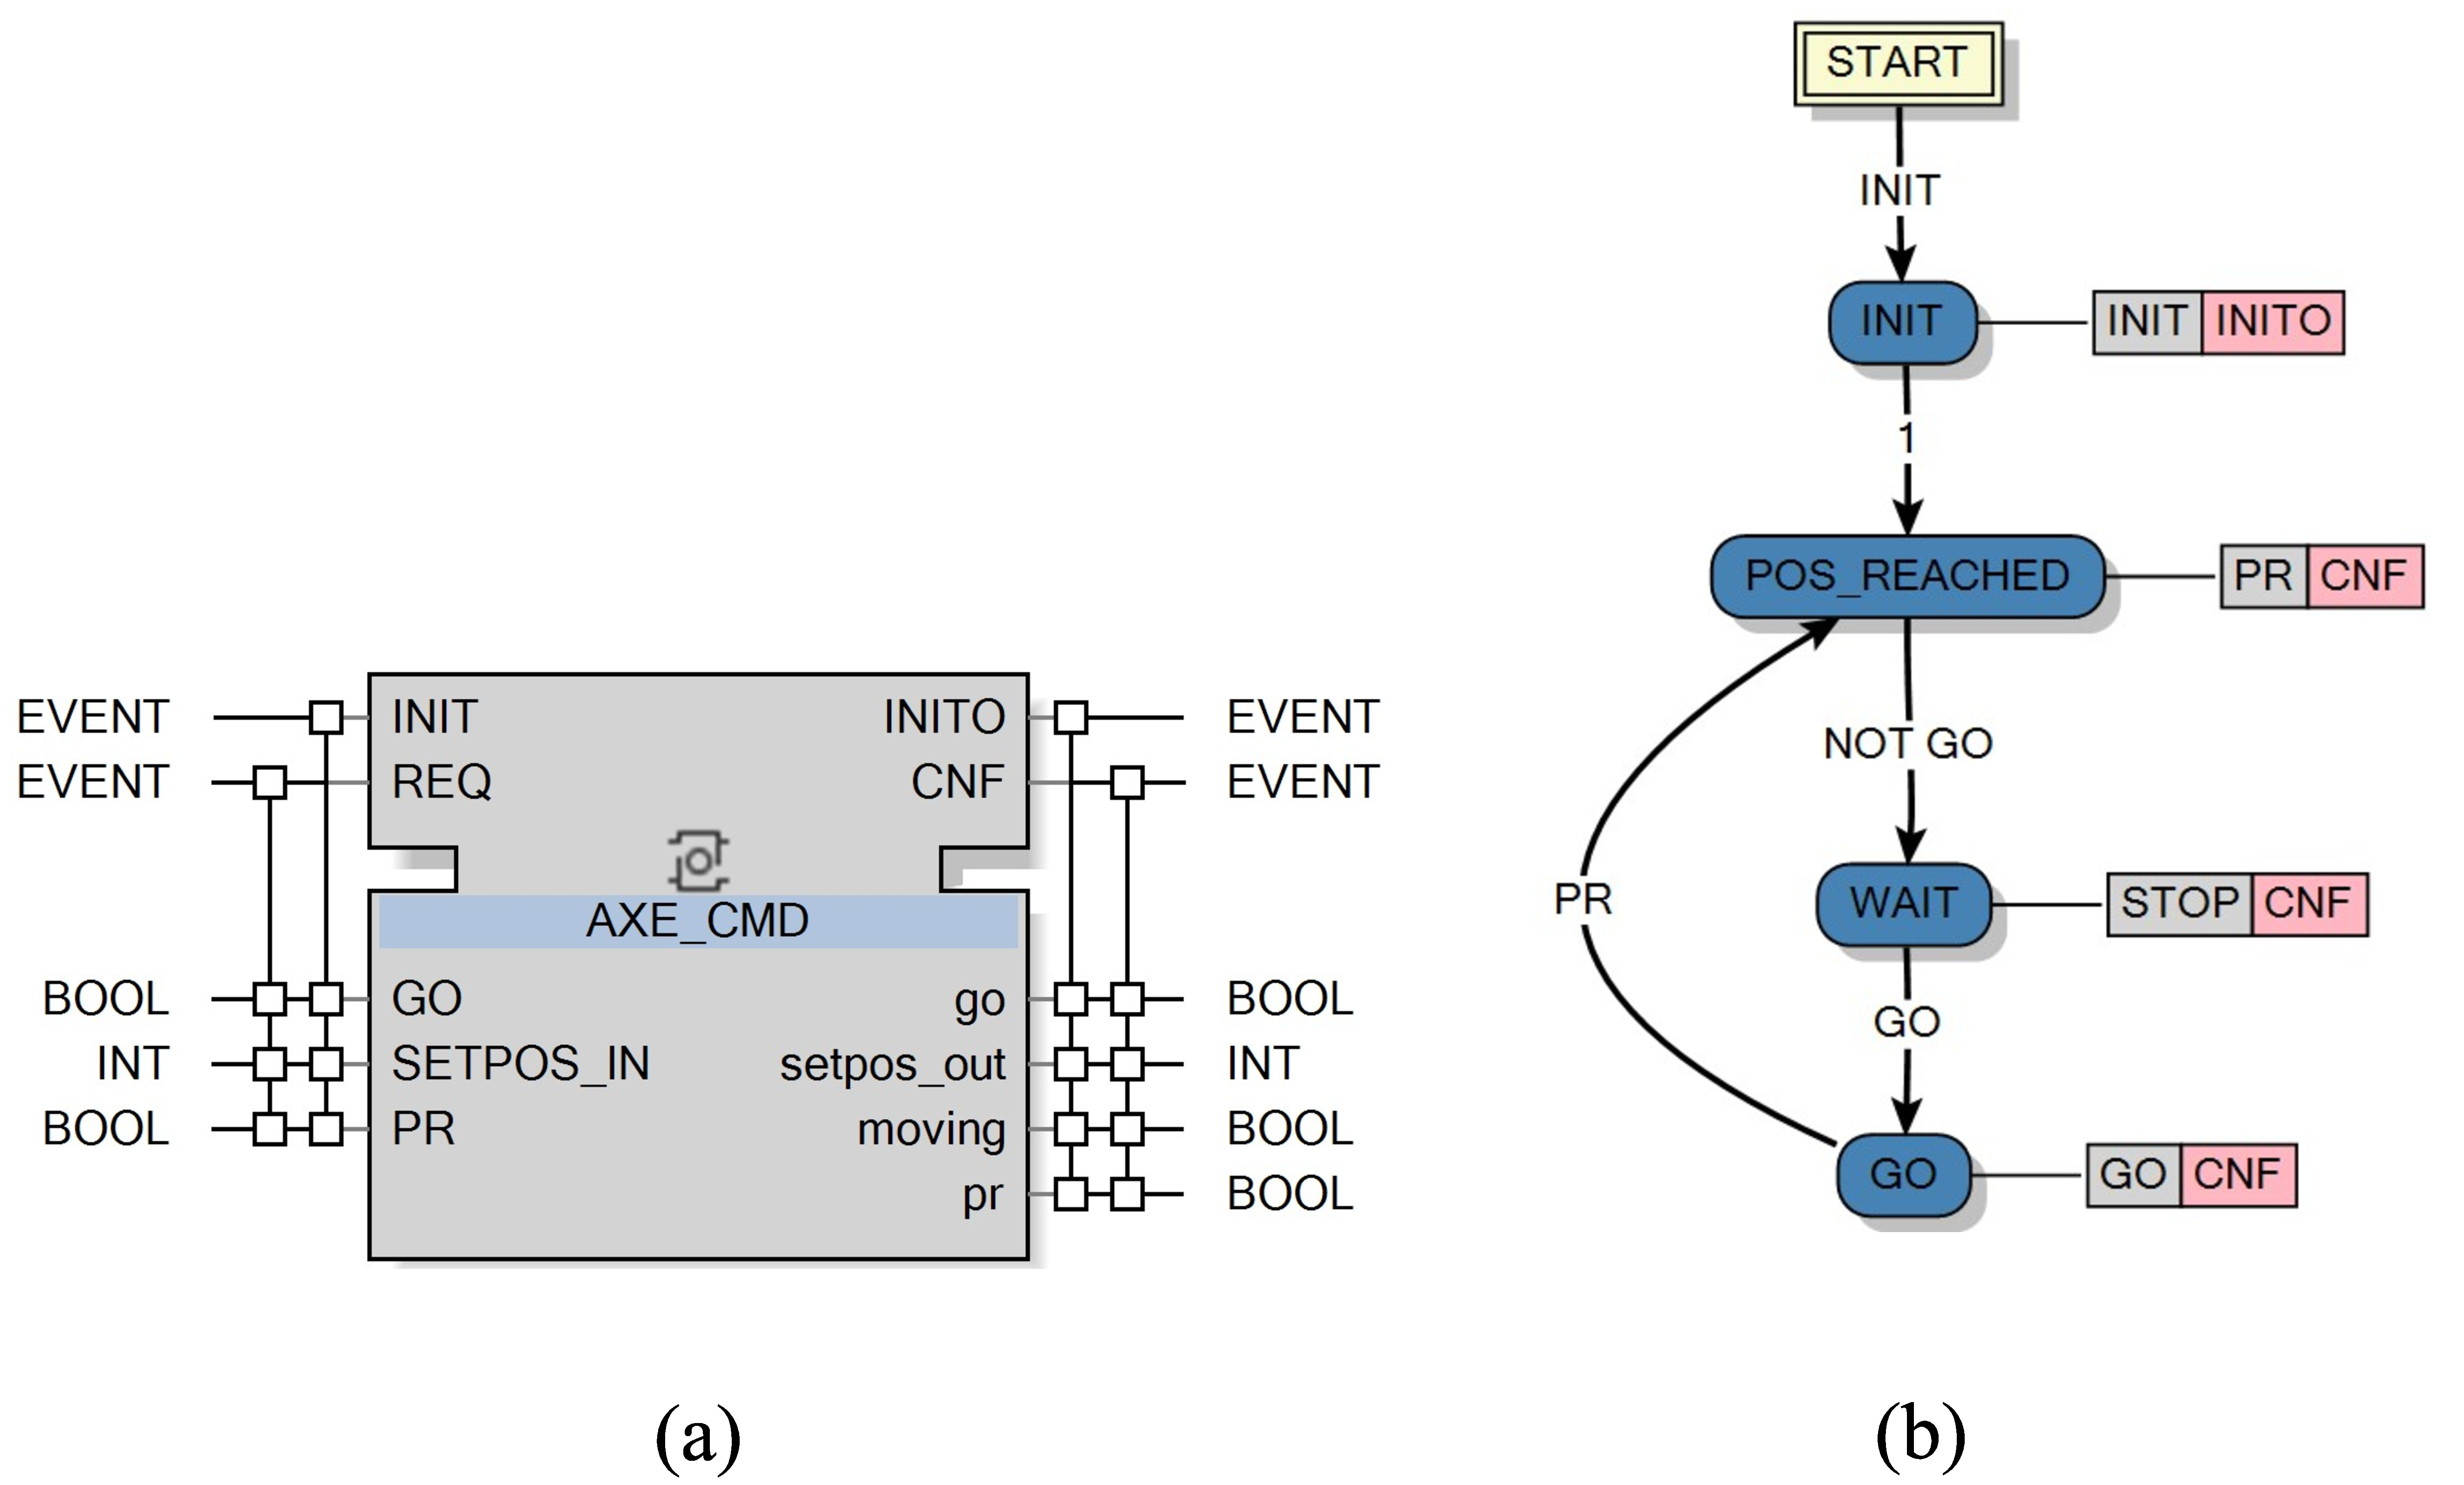
\includegraphics[width=0.9\columnwidth]{MX_Papers/Paper4/pictures/lilli06.eps}
    \caption{Overview of the controllers dedicated to the HHM linear motion axes and gripper. (a) The AXE\_CMD FB, (b) the AXE\_CMD ECC.} 
    \label{fig:fbs}
\end{figure}

\subsubsection{Linear motion axes}
A standardized pair of controller and plant Function Blocks can be used to conceptually model the three linear axes.
Using a modular and reusable strategy, the development work can be significantly decreased. 
Additionally, it makes it possible for the system to be easily reconfigured in order to achieve alternative capabilities in the future.
The core Function Block \codeword{AXE_CMD}, which implements an absolute positioning control system, is shared by the three linear axes. The FB and the correspondent ECC are displayed in \mbox{Fig. \ref{fig:fbs}}.
The plant FB precisely sets the axis according to the destination coordinates and provides the \codeword{POS_REACHED} signal to the controller once the motion is completed.
The given target position directs the \codeword{AXE_CMD} to the preset coordinates. The FB acknowledges its arrival and stops it once it reaches the designated spot. A visual representation of the \textit{elevator} linear motion axis is reported as an example in Fig. \ref{fig:elevator}.

% Figure: elevator
\begin{figure}[h!]
    \centering
    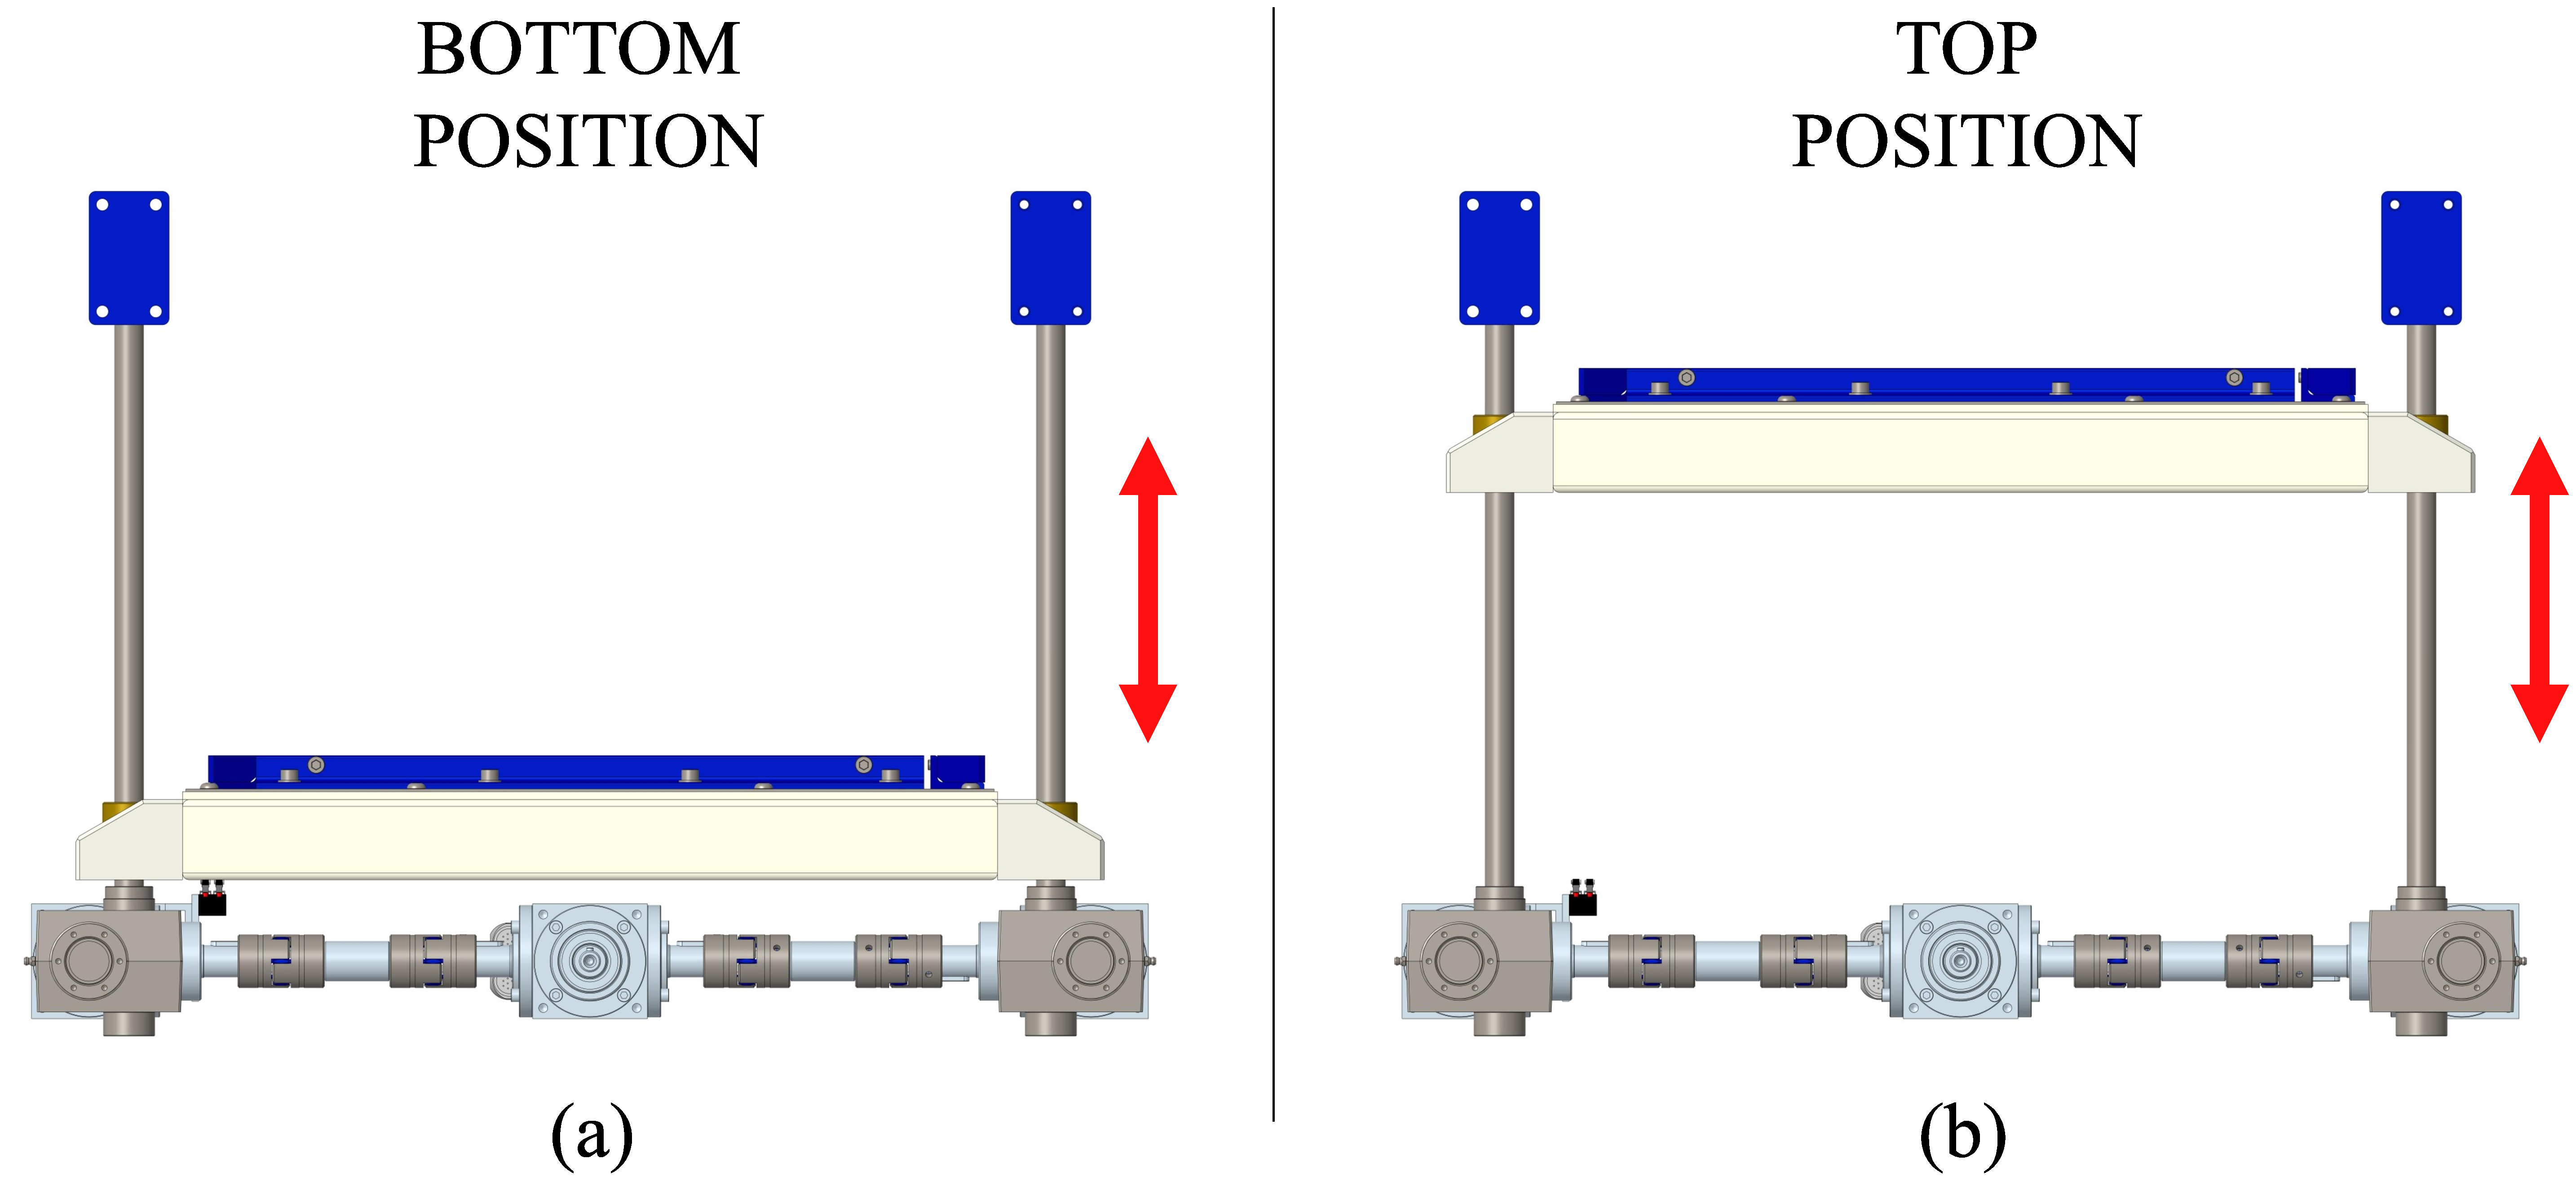
\includegraphics[width=\columnwidth]{MX_Papers/Paper4/pictures/lilli07.eps}
    \caption{Visual representation of the elevator linear motion axis: (a) bottom position, (b) top position. } 
    \label{fig:elevator}
\end{figure}

\subsubsection{Gripper}
The operating mode of the HHM pneumatic \textit{gripper} differs from the above-mentioned systems due to its inherent discrete logic. 
\textit{Gripper} \codeword{CLOSE} or \codeword{OPEN} commands are processed when the \codeword{REQ} event is triggered. The FB provides two output signals to indicate when the relevant \quotes{closed} or \quotes{open} state has been reached. 

\subsubsection{Sequence Controller}
The \codeword{SEQUENCE} FB manages the integration of the various subsystems and the overall HHM behavior throughout the execution of the remote handling sequence. The precise list of tasks is defined within the correspondent ECC. 
Each FSM state is associated with a set of actions carried out by a specific algorithm. Motion actions are started by setting the desired position for a specific axis and sending the \codeword{GO} command to the appropriate controller. The reception of the \codeword{POS_REACHED} command from the plant Function Block causes the transition to the next state. In our case study, the sequence controller Function Block implements a state machine that refers to a single HHM task: the TIS unit pick-up sequence. This sequence has been examined as a representative example. The system's adaptable architecture will make it possible to incorporate more motion sequences in the future by updating a single Function Block.

\subsubsection{Support Function Blocks}
The \codeword{INIT} Function Block initializes the system and prepares it to perform the desired procedure at the start of software execution.
The user can then choose between manual and automatic HHM operating modes by using the \codeword{TRIGGER} and \codeword{MODE_SELECTION} Function Blocks.
While the first allows the user to direct the HHM behavior, the automatic mode forces the system to stick to the Sequence controller's state machine logic.
The \codeword{ESTOP} Function Block, as the last support FB, offers the ability to stop the execution at any time. This feature protects the system from internal or external failure caused by unfavorable conditions.

\section{Simulation Model}
\label{sec:simulation}
IEC 61499 applications can typically be tested using dynamic (online) or static (offline) techniques. In order to assure safety in a system that has already been deployed and is in use, the first group of techniques seeks to monitor it in its operating state. Conversely, offline safety measures are meant to reduce fault risk at the design stage and test the system before use \cite{Ovsiannikova2021b}.
In our work, we focused on offline verification methods aimed at fault removal. 
This process can be accomplished at the designed stage using formal verification tools or online testing techniques. 
Software simulation involves feeding the program with input sequences that replicate the behavior of the actual system and determining whether or not the program's outputs comply with specific requirements.
The adopted development suite includes a native Human Machine Interface (HMI), which may be used as a command center and to simulate system execution.
Composite Automation Types (CAT) were used to model a range of mechatronic components for the simulated plant. This feature facilitates testing of the system's simulation behavior in a common environment because CATs can be directly linked to both HMI objects and Function Blocks.
Inputs were used to link the controller Function Blocks to the relevant CAT blocks, replicating the real-world behavior of the mechatronic components in the system. The HHM representation implemented in the HMI is shown in \mbox{Fig. \ref{fig:hmi}}, where the three linear motion axes are linked to distinct CAT blocks. 
Each axis plant FB is connected to a dedicated \codeword{AXE_CMD} controller, which selects the desired position set-point from a predefined pool of coordinates and triggers the motion request. In response to the controller's inputs, the plant block validates the coordinates, performs the movement, and acknowledges its arrival at the predetermined location. The axis motion may be stopped at any time by activating a \codeword{STOP} input event.
The \codeword{GR_CMD} FB opens or closes the clamp based on the input signal from the controller. In order to interlock the option of releasing the payload only in particular positions, the \codeword{GR_CMD} is additionally provided with the axes' actual positions.

We should emphasize that the HMI CATs provide a more accurate representation of the system behavior when compared to the axis plant Function Blocks discussed in \mbox{Sec. \ref{sec:case_study}}. While in the basic implementation, the plant FB will only trigger the \codeword{POS_REACHED} signal after an arbitrary time, here an integrator simulates the linear axis movement and sends the actual position coordinates to the correspondent object in the HMI allowing the user to follow the motion while it is being executed. Further debugging tools, such as runtime monitoring blocks, can be also employed to detect specific critical conditions.
The software's modularity allows for the independent and concurrent development of the controller and plant Function Blocks. Each FB will be initially tested and debugged with the aid of custom mock-up blocks. As they reach maturity, they can then be interconnected to run the simulation. After the verification, the final stage will be to replace the simulation's plant FB with the actual system. 

Unfortunately, simulations often cannot explore all possible paths due to the huge size of state automata representing industrial control software. This bottleneck makes them insufficient as an exhaustive verification method since it prevents conclusive verification of program behavior in a reasonable amount of time. Furthermore, the quality of the output is also influenced by the automation engineer's knowledge and experience in selecting pertinent testing sequences that may correspond to typical dangerous circumstances of the controlled process \cite{Schnakenbourg2002}. 
To address these problems, formal verification techniques have been established, which provide methods for closed-loop (plant and controller) model checking able to analyze a program in its entirety.

% Figure: hmi
\begin{figure}[h!]
    \centering
    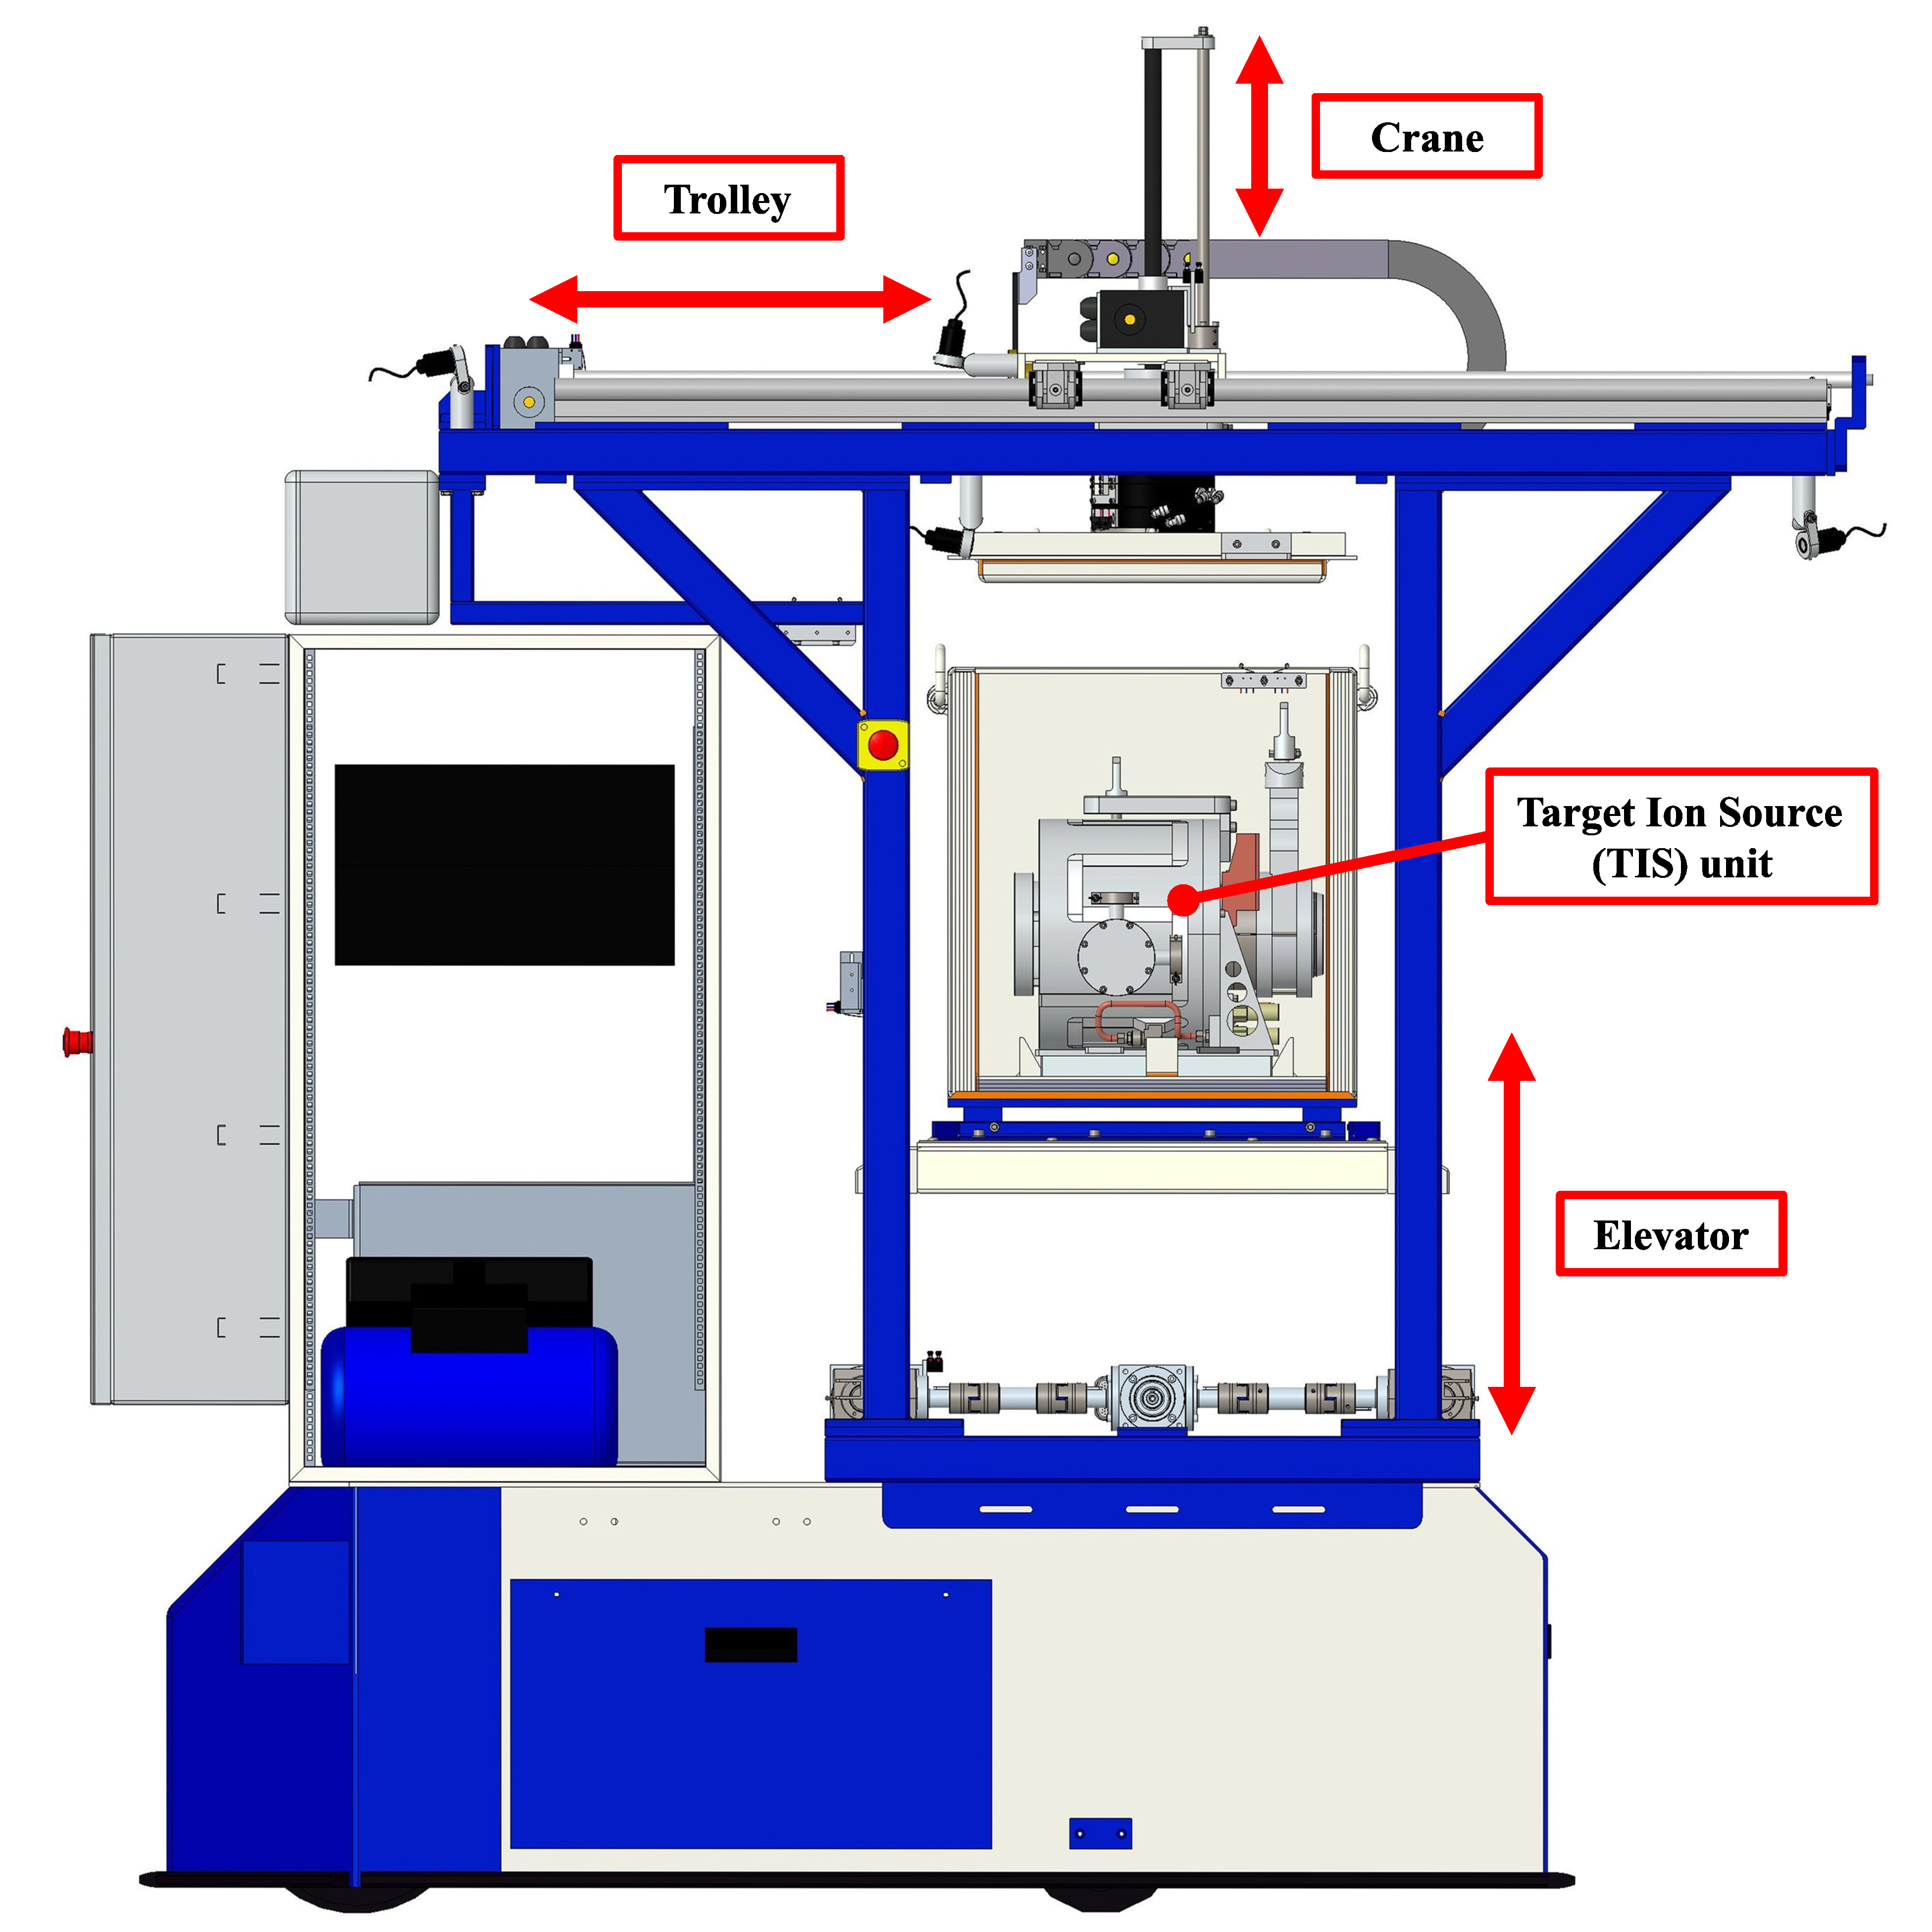
\includegraphics[width=\columnwidth]{MX_Papers/Paper4/pictures/lilli08.eps}
    \caption{Graphical representation of the HHM Composite Automation Type (CAT) used in the Human Machine Interface (HMI) for online monitoring and simulations.} 
    \label{fig:hmi}
\end{figure}


% Table: 1 
\begin{table*}[!hb]
    \centering\small
    \renewcommand{\arraystretch}{1.5}
    \begin{tabularx}{\textwidth}{ m{0.1\textwidth} m{0.4\textwidth} m{0.4\textwidth} }
        \hline
        No & Property & Comment                                                                         \\ 
        \hline
        1   & \texttt{G !(ELplant.POS\_OUT = 5)} &  
        The \textit{elevator} plant Function Block must never reach the \textit{error} state in any of the sequence elements.                                                 
        \\ 
        2   & \texttt{G !(CAplant.POS\_OUT = 5)} &  
        The \textit{trolley} plant Function Block must never reach the \textit{error} state in any of the sequence elements.                                                       
        \\ 
        3   & \texttt{G !(CRplant.POS\_OUT = 5)} &                                                    The \textit{crane} plant Function Block must never reach the \textit{error} state in any of the sequence elements.                                                       
        \\ 
        4   & \texttt{G !(CRplant.POS\_OUT in (2..4) \& CAcmd.moving = TRUE)} &                       
        The \textit{crane} must always be in the top position while the \textit{trolley} is moving to prevent mechanical collisions.
        \\      
        5   & \texttt{G !(ELplant.POS\_OUT = 2 \& CRplant.POS\_OUT = 4 \& CAcmd.moving = TRUE)} &     
        To avoid mechanical collisions, the \textit{trolley} must not move while the HHM is lowering the TIS unit inside the HHM shielding box.      
        \\ 
        6   & \texttt{G !(ELplant.POS\_OUT = 1 \& CRplant.POS\_OUT = 4 \& GRplant.GRO = TRUE)} &      
        The pneumatic \textit{gripper} shouldn't open until the \textit{elevator} is not in the top position, even if the \textit{crane} is in the lower position.       
        \\ 
        \hline
    \end{tabularx}
    \caption{Description of the LTL specifications verified with NuSMV in the HHM model.}
    \label{table:1}
\end{table*}

% Figure: par_seq
\begin{figure*}
    \centering
    
\includegraphics[width=\textwidth]{MX_Papers/Paper4/pictures/lilli09.eps}
    \caption{A comparison of the two investigated control sequences. (a) illustrates the ECC of the Controller FB implementing the parallel movement of the three linear axes, whereas (b) shows the ECC in which the three movements are executed sequentially.} 
    \label{fig:par_seq}
\end{figure*}

\newpage

\section{Formal verification}
\label{sec:formal_verification}
The formal verification of finite state systems, such as \mbox{closed-loop} control algorithms, has been effectively accomplished in the last ten years thanks to symbolic model checking based on Binary Decision Diagrams (BDDs). These tools have been developed in the past to overcome the state explosion problem in finite automata \cite{burch1992}. 
Model checking is the process of exploring the reachable states of a model, which is described as a finite state machine, in order to validate temporal logic specifications.
When a property is violated, the tool provides a counterexample in the form of a sequence of states \cite{Biere2003}. As previously mentioned, the most well-known open-source model detection tools among the available solutions are NuSMV and SPIN. In particular, because of its extensive core capabilities and good scalability, NuSMV is frequently used for reliability and security verification of industrial designs \cite{xu2018}. This tool supports the representation of synchronous and asynchronous finite state systems and it allows for the verification of both Linear Temporal Logic (LTL) and Computation Tree Logic (CTL) specifications using implicit methods. In more detail, it compares a model against a property using a symbolic representation of the specification \cite{frappier2010}. 

Accurate modeling of the real system is essential in order to validate the  intended behavior of the device and detect potentially undesirable states. This enables simulation and verification of the apparatus prior to its actual operation. Since the model is an abstraction, it may not include all relevant characteristics of the real-world system or the context in which it is embedded. Hence, a condensed version of the plant FB can be used to create a reduced formal model, which can then be verified utilizing symbolic model checking techniques thanks to the NuSMV tool.
As an illustration, in the presented use case, the \codeword{AXE_CMD} FB only takes into account the beginning, intermediate, and final states rather than the motion dynamic considered in the real system. 
This approximation is still acceptable because the goal at this stage is to assess the possible blockage within two locations instead of the specific stop positioning. 

Table \ref{table:1} describes a collection of LTL expressions that have been developed to identify potential critical problems.
Specifications 1-3 are meant to ensure that none of the three linear motion axis plants enters the error state during system execution. On the other hand, requirements 4 and 5 deal with potential collision detection. More in detail, the first verify that \textit{trolley} movements are inhibited when the \textit{crane} is not fully raised in the top position, and the second focuses on the system configuration occurring while positioning the TIS unit within the shielding box. Similarly to the last scenario, the \textit{trolley} must not move while the \textit{elevator} is raised and the \textit{crane} is lowered.
Specification 6 aims to confirm that the \textit{gripper} only opens in a specific location: when the TIS unit is lowered within the box (\textit{elevator} up and \textit{crane} down). 
A batch script, detailed in Appendix \ref{appA:NuSMV script}, has been developed to examine all the aforementioned requirements with NuSMV and log data.

The LTL specifications were evaluated in two different scenarios to test the reliability of the formal verification. 
As described in Section \ref{sec:case_study}, the \codeword{SEQUENCE} FB implements a FSM where the HHM axis movements are executed sequentially to prevent any potential collision. 
If we specifically consider state \codeword{GRC_03_GRC_04} in Fig. \ref{fig:par_seq}, which corresponds to the TIS unit picked up by the HHM cartesian manipulator, the subsequent path towards the shielding box shall be carried out in three distinct steps: (1) Backward movement of the \textit{trolley} axis, (2) lowering of the \textit{crane} axis, and (3) rising of the \textit{elevator}. The described motion sequence and the correspondent states are visible in \mbox{Fig. \ref{fig:par_seq} (b)}.
In our research, we deliberately induced a design flaw in the control software to determine if NuSMV was able to identify it. 
Specifically, we updated the main FSM to launch the previously mentioned actions in a parallel execution, with the three motion axes moving simultaneously, as shown in \mbox{Fig. \ref{fig:par_seq} (a)}. 
Since it does not always result in a fault condition, this type of design error is particularly difficult to identify through conventional simulations. 
The relative motion axes speeds do, in fact, affect the likelihood of a collision. This implies that we may be able to perform multiple simulations without observing any failure event. The following section discusses how adding non-determinism to the model can make it more realistic by taking into account the impact of non-idealities found in the real world and allowing for the early identification of potential system defects.
With regard to the test under discussion, NDTs within axes plant FBs seek to change the amount of time required to get the \codeword{POS_REACHED} signal, directly impacting the relative speed between concurrent axis movements.
The violation of LTL specification No. 5 in Table \ref{table:1} allows for the detection of the collision occurrence. 

\subsubsection*{Discrete State Plant Modelling in Function Blocks with Non-Deterministic Transitions}
The original system, created to exploit the visualization and online verification capabilities provided by EcoStruxure\textsuperscript{\texttrademark} Automation Expert, needs to be reduced and adapted in order to apply formal verification methods. The \textit{elevator}, \textit{trolley}, and \textit{crane} components were modeled in this study by a simplified Function Block that embodies the intended behavior of the actual system while omitting the features used for visualization. As opposed to the simulation scenario where each component was modeled using a single Function Block, this global plant model has been implemented to capture the behavior of the three linear motion axes collectively.
Thus, by discretizing the plant model's Function Block while maintaining its functional capabilities, the original complex model can be reduced to a simpler representation.
The \codeword{AXE_PLANT} component features two data inputs (\codeword{GO} and \codeword{POS_IN}) and two data outputs (\codeword{POS_REACHED} and \codeword{POS_OUT}).
The system may simulate real-world behavior using the non-deterministic transition (NDT) event's random signal emission, which enables the discovery of previously undetected faults using CTL or LTL specifications.
As an example, Fig. \ref{fig:ndt} depicts a potential scenario in which a NDT has been introduced in the ECC associated with \textit{elevator} plant FB.
In this case the plant enters the \codeword{GO} state upon receiving the controller's \codeword{GO} signal and following the NDT event, it reaches the \codeword{END} state.
The physical meaning of this NDT is that the transition between the \codeword{GO} and \codeword{END} states, i.e. the axis motion towards a given position, might take an unspecified amount of time.
If a \codeword{NOT_GO} signal is generated while the plant is in the \codeword{GO} state, it enters the \codeword{STOP} state and remains there until another \codeword{GO} signal is activated.
In the \codeword{END} state, the plant notifies the controller that the task has been completed by setting the value of  \codeword{POS_REACHED} signal to \codeword{TRUE}. 
Following the deactivation of the \codeword{GO} signal, the plant returns to the \codeword{HOME} state.

% Table: 2
\begin{table}[b!]
    \centering\small
    \renewcommand{\arraystretch}{1.5}
    \begin{tabularx}{\columnwidth}{ m{0.1\columnwidth} m{0.9\columnwidth} }
        \hline
        No. & Scenario                                                                                   \\ 
        \hline
        1   & NDT in \textit{elevator} plant                                                            \\ 
        2   & NDT in \textit{trolley} plant                                                             \\  
        3   & NDT in \textit{crane} plant                                                               \\ 
        4   & NDT in \textit{gripper} plant                                                             \\ 
        5   & NDT in \textit{elevator} and \textit{trolley} plants                                      \\ 
        6   & NDT in \textit{elevator}, \textit{trolley} and \textit{crane} plants                      \\ 
        7   & NDT in \textit{elevator}, \textit{trolley}, \textit{crane} and \textit{gripper} plants    \\
        \hline
    \end{tabularx}
    \caption{Non-Deterministic Transition (NDT) scenarios analyzed in the study: NDTs are progressively included in the model.}
    \label{table:2}
\end{table}

% Figure: ndt
\begin{figure}[t!]
    \centering
    \includegraphics[width=0.95\columnwidth]{MX_Papers/Paper4/pictures/lilli10.eps}
    \caption{Example of injection of a Non-Deterministic Transition (NDT) within the elevator plant model.}
    \label{fig:ndt}
\end{figure}

% Figure: fbme
\begin{figure*}
    \centering
    \includegraphics[scale=0.5]{MX_Papers/Paper4/pictures/lilli11.png}
    \caption{FBME trace analysis.} 
    \label{fig:fbme}
\end{figure*}

\noindent The \textit{gripper} plant model features two data inputs, \codeword{OPEN} and \codeword{CLOSE}, and two data outputs, \codeword{GRO} and \codeword{GRC}. 
The model initially enters the \codeword{OPENING} state when the controller sets \codeword{OPEN} to \codeword{TRUE}. Second, it switches to the \codeword{OPEN} state in response to a NDT signal.
Similarly, when the controller sets \codeword{CLOSE} to \codeword{TRUE}, the plant reaches the \codeword{CLOSING} state and, following a random time delay caused by the NDT, enters the \codeword{CLOSED} state.
If the \codeword{CLOSE} command is activated during the \codeword{OPENING} state, the model transitions to the \codeword{CLOSING} state. If the \codeword{OPEN} command is activated during the \codeword{CLOSING} state, the plant returns to the \codeword{OPENING} state and awaits for the emission of the NDT signal.
The discrete state model of the HHM was converted into an SMV model using the FB2SMV tool. Subsequently, the verification has been carried out by NuSMV, using an Intel\textsuperscript{\textregistered} core\textsuperscript{\texttrademark} \mbox{i7-10510U} CPU@1.80 GHz 2.30 GHz with 32 Gb RAM. 
In an effort to mitigate the state space explosion problem, NDTs have gradually been introduced into different sections of the model according to the scenarios in Table \ref{table:2}.
The progressive integration of NDTs might be viewed as a feature of the proposed tool-chain.
While it is true that critical faults might occur as a result of multiple non-deterministic conditions acting simultaneously, in a first verification stage, distinct blocks can be assessed independently while maintaining the execution time within reasonable limits. 

\subsubsection*{Trace analysis using Function Blocks Modelling Environment (FBME)}
In our work, we used Function Blocks Modelling Environment (FBME) \cite{FBME}, enhanced with trace visualization and in-depth analysis capabilities, to examine counterexamples and find the causes of violations of requirements. 

One of the non-trivial tasks when using formal verification is to analyze the resulting counterexample. Verifiers frequently offer an output trail in a text format that is inconvenient and confusing to the user. As a result, the user has to make additional efforts to analyze the counterexample. 
The IEC 61499 code presents additional challenges due to the automatic generation of the model for the verifier, which leads the counterexample to utilize the notations of the input model. 
Given an output trace, the following natural step is to determine the location of the error and investigate the underlying causes. The non-imperative nature of IEC 61499 further complicates this process. Moreover, current common IEC 61499 software development tools do not provide in-depth trace analysis capabilities. 

FBME is an Integrated Development Environment (IDE) for IEC 61499 applications, currently under active development at Luleå University of Technology (LTU). FBME is a cross-platform, open-source, modular IDE that is based on IntelliJ IDEA and the Meta Programming System (MPS) \cite{mps}. MPS provides powerful tools for developing custom Domain-Specific Languages (DSL) and also provides a platform for creating custom IDEs. Modularity and extensibility are key features of FBME, so LTU has also extended FBME's functionality by adding enhanced capabilities to the visualization and automatic analysis of IEC 61499 program execution traces and counterexamples. 
The functionality to automatically call NuSMV and generate a model for verification was also seamlessly integrated into FBME.

\newpage

\noindent The trace analysis in FBME is shown in Fig. \ref{fig:fbme}. Trace is stored in unified format \cite{liakh2022formal} and can be obtained from different sources: either from a simulation of the verifier model, as a counterexample, or from the actual execution of the IEC 61499 program. The entire trace history is displayed on \mbox{panel 1}. The user selects the trace step of interest and can examine the state of the system. The values of all variables, message counters and other data are also displayed on the diagram itself (2), where changes that have occurred in the current step are highlighted. 
In addition to clear visualization of the trace, FBME uses powerful techniques for its in-depth analysis. 
By examining the preceding code, this method enables the user to visually locate the section of the code that resulted in the problem. 
Visual Explanation allows to establish causal relationships between different trace events (note that the term  \quotes{event} here is used in a broader sense, as a change in system state, rather than an event in IEC 61499 terms). For instance, it might be possible to determine whether a variable modification, an IEC 61499 event emission, or a change in an ECC state produced a specific event. 
In this way, the cause of the violation of a requirement can be identified. An example of the result of Visual Explanation technique is available in window 3.

% Figure: graph
\begin{figure*}
    \centering
    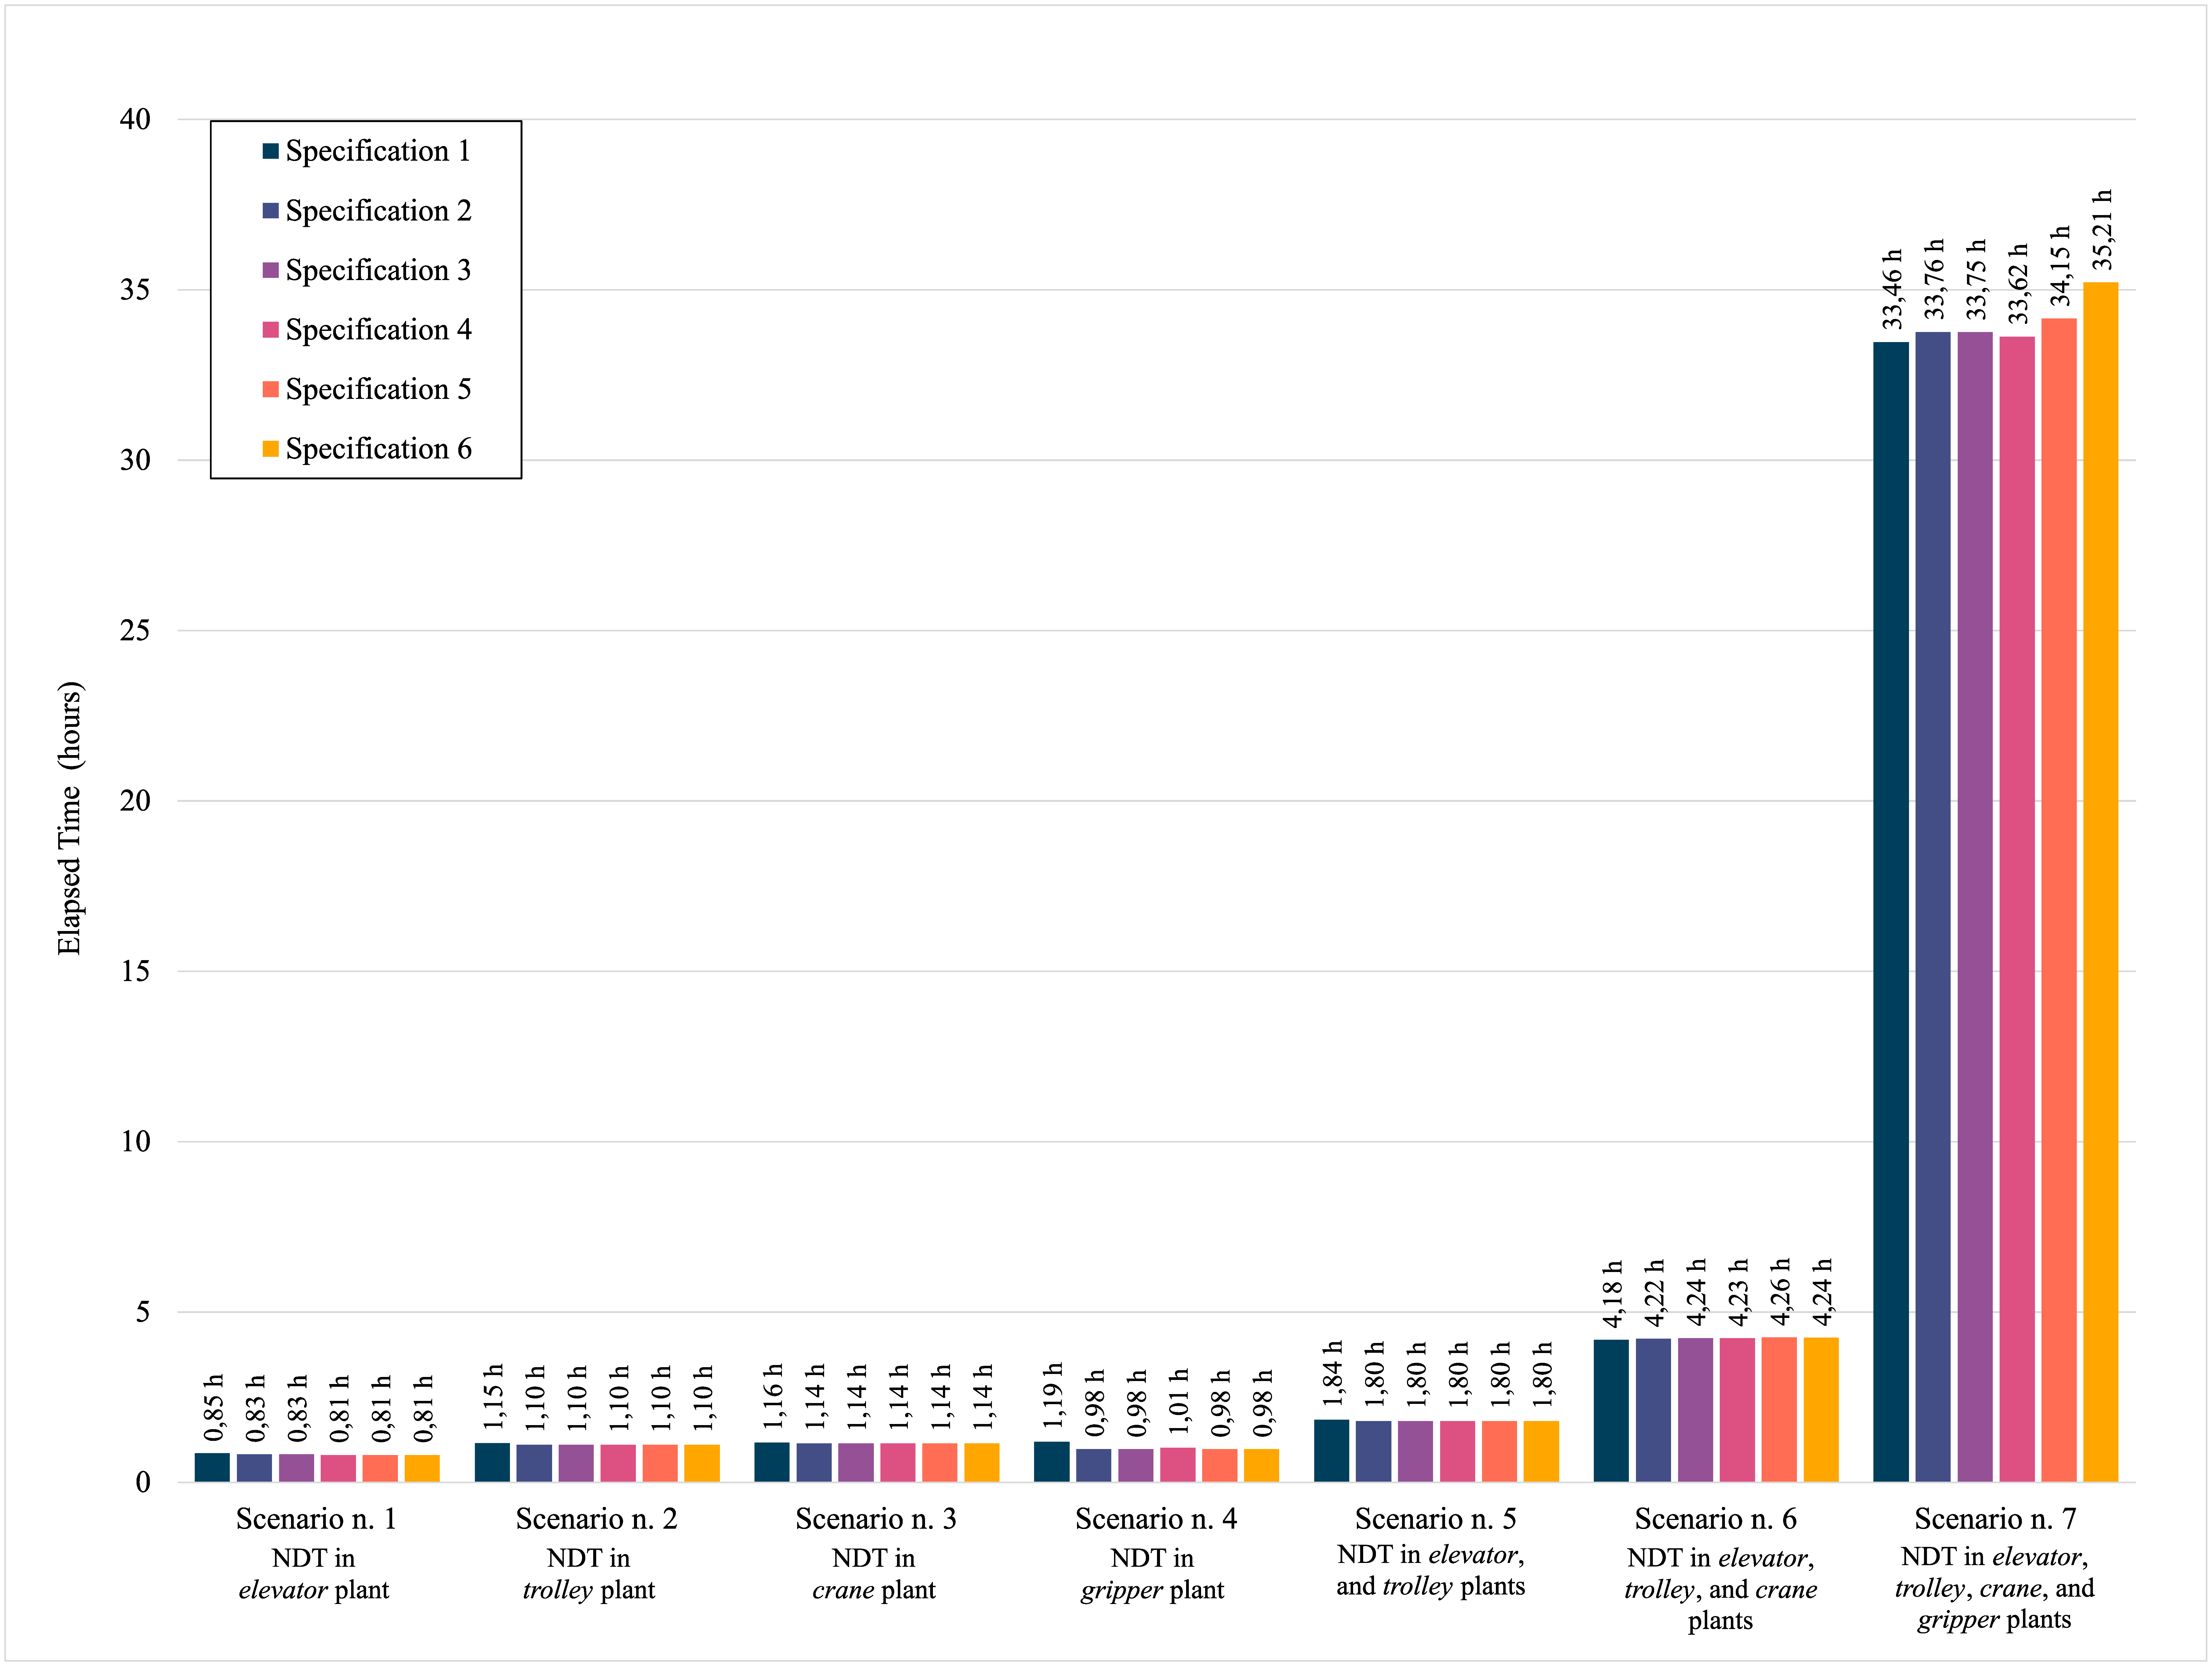
\includegraphics[width=0.84\textwidth]{MX_Papers/Paper4/pictures/lilli12.eps}
    \caption{Execution time required by NuSMV in different NDTs configuration.} 
    \label{fig:graph}
\end{figure*}

\section{Results and Discussion}
\label{sec:results}
The initial phase of the project, which followed the software remodeling based on IEC 61499, was devoted to validating the model by launching various simulations directly within the EcoStruxure\textsuperscript{\texttrademark} Automation Expert suite.
This was achieved through the use of CATs, which allow Function Blocks to be directly linked to HMI objects.
The application model and the HMI have been developed independently. Once sufficiently stable, the HMI plant FB was connected to the controller FBs, replacing the existing simplified version of plant FBs.
Launching the online simulation, the user can monitor the sequence execution. The software will begin in the initial state, progress through specific checkpoints, and eventually reach the final state.
Unfortunately, even if the simulation doesn't report any errors, this merely indicates that there exists a path where it crosses all the checkpoints.
Hence, using symbolic model checking tools will provide a more thorough level of investigation.
Prior to the verification procedure, it is crucial to verify the accuracy of the formal model. This can be accomplished by simulating the model in NuSMV, where various paths and random states are explored.
The simulation assists in demonstrating that the model properly covers all the ECC states of the behavioral Function Block by tracing the path of ECC states. It also helps to confirm that the generated formal model behaves in accordance with the discrete state model by providing information about the values of all the variables in each state.
The NuSMV simulation technique can detect changes in the ECC and their impact on system behavior.
Initially, using this method it will be possible to confirm that all paths leading from the beginning to the end will pass through the crucial checkpoint. As the second step, this assertion needs to be proven even in the presence of non-determinism.
Indeed, the introduction of NDTs may have resulted in the inclusion of certain additional pathways in the application, and this is reflected in a larger state space with multiple routes. In contrast to simulation, where we can test only one scenario, NDTs allow us to evaluate several possibilities. The evidence that the given specifications are validated in all of these paths will thus extend the results of the online simulation. The six formulated properties have been checked using a batch script that reads the supplied SMV model and performs the verification, logging both the execution time and result for each specification. 
The quantity of memory needed to store and manipulate BDDs is the primary limitation of model checking methods. In light of this, the proposed implementation allows for the gradual integration of NDTs into the model. This stepwise approach provides better control over the model and allows for faster specification analysis. The time required for NuSMV to execute the formal verification of all the described LTL specifications while altering the number of NDTs is depicted in Fig. \ref{fig:graph}. It is evident that the gradual inclusion of NDTs resulted in a global increase in execution time.
Because of the ample state space, it is feasible that with a larger number of NDTs, global verification of all pathways will fail.
Reducing the number of NDT points in this situation may be a viable option for squeezing the state space to a tolerable size and then gradually increasing it.
Bounded Model Checking (BMC) is an alternate strategy that searches for a counterexample in executions whose length is constrained by some number k. If no bug is discovered, k is increased until either a bug is discovered, the problem becomes unmanageable, or some predetermined upper bound is reached \cite{Biere2003}.
A key feature of the described engineering framework is the ability to govern non-determinism. NDTs can be injected into specific locations to perform formal verification in a particular configuration. This method allows us to validate the automation system under particular stress conditions.
As discussed in Section \ref{sec:formal_verification}, the IEC 61499 application was formally verified following the purposeful introduction of a design fault that might potentially lead to a collision occurrence.
Despite the difficulties in identifying this failure condition using conventional simulations, NuSMV was able to successfully accomplish this task, thus providing a counterexample which demonstrates the violation of LTL property No. 5 in Table \ref{table:1}.
In the case under study, the amount of time needed for the formal verification was comparable with what was required for the same LTL expression in Scenario No. 7 (see \mbox{Fig. \ref{fig:graph}}). However, it is difficult to formulate a generic statement because the duration depends on the particular paths that lead to the failure conditions. 
The evidence of the violation is provided by NuSMV in the form of a failure trace, which depicts a state sequence of system model transitions where the specification is not met. \mbox{Figure \ref{fig:counterexample}} shows how, through the use of specific visualization tools \cite{pakonen2018} it would be possible to decode the output trace and examine the path that led to the violation. 
This result is of great significance as it showcases how the presented set of tools can be employed in the verification of complex safety-critical control systems, enabling the early detection of potential failure conditions that would be extremely difficult to spot through traditional simulation and testing techniques. 

% Figure: counterexample
\begin{figure}[t!]
    \centering
    \includegraphics[width=\columnwidth]{MX_Papers/Paper4/pictures/lilli13.eps}
    \caption{Graphical visualization of the counterexample trace produced by NuSMV when a LTL specification is violated.} 
    \label{fig:counterexample}
\end{figure}

\section{Conclusions and Future Work}
\label{sec:conclusion}
In this paper, we've shown how to use an integrated tool-chain for the analysis and verification of the control software for a real, safety-critical automated system employed in the transport and storage of radioactive material in a nuclear research facility. 
The provided use case was intended to demonstrate the actual feasibility of integrating the phases of modeling, simulation, verification, and analysis in a complex system using an automatic procedure.
The study benefited from the software redesign based on the IEC 61499 standard for several kinds of reasons.
First, it enabled the optimization of code structure by defining standardized, modular, and reusable FBs based on specific ECCs. Second, it allowed for the explicit specification of the relationships and dependencies between FBs while eliminating the incorporation of global variables. Third, it supported the translation of the code into an SMV model, thereby enabling formal verification of LTL safety specifications. Finally, the incorporation of NDTs within different Function Blocks facilitated the simulation of sequence execution under realistic conditions. 
The developed IEC 61499 solution's portability promotes the system to be integrated into various tool-chains. In the proposed example, we investigated this feature by combining it with FB2SMV and FBME for the verification of a set of LTL safety specifications. 
While the first tool is used to extract the software formal model, model verification is subsequently carried out using NuSMV. FBME, on the other hand, is a comprehensive tool, capable of automating the entire verification process by incorporating automatic model generation, NuSMV verification, visualization, and analysis of counterexample trace.
The suggested tool-chain can be instrumental in the early identification of design flaws that could result in potential mechanical collisions. The presented results emphasize the validity of the tool-chain by demonstrating the benefits of formal system verification in detecting non-trivial design errors that may result in a failure event under specific circumstances.
A key feature of the proposed solution, in addition to modularity and portability, is the deep control over localized NDT introduction. This capability can be effective in reducing the process complexity, permitting independent testing of specific FBs, and keeping the time required by model checking within reasonable limits. 
One limitation of the presented methodology resides in the accuracy with which the IEC 61499 model represents the actual system. Indeed, the necessity for mitigating the state explosion problem ultimately led to the adoption of a simplified design, especially with regard to plant FBs. 
Ensuring a high level of accuracy between the model and its real-world equivalent is crucial during this phase. Furthermore, in the provided use case we investigated a single, albeit critically important, remote handling procedure. 
Further developments will allow the software model to be expanded to include more system motion sequences and plant details, thus finalizing the development of a digital twin of the primary SPES remote handling system.

%\section*{Acknowledgment}

\section*{Appendix A: NuSMV script}
\label{appA:NuSMV script}
\begin{figure}[h!]
    \centering
    \begin{lstlisting}[caption=Batch script used to check the LTL specifications with NuSMV.]
    time
    read_model -i HHM_FV_PART_1.smv
    flatten_hierarchy
    encode_variables
    build_model
    time
    check_ltlspec -p "G !(HHM_FV_PART_1_inst.ELplant.POS_OUT = 5)" -o spec1.txt
    time
    check_ltlspec -p "G !(HHM_FV_PART_1_inst.CAplant.POS_OUT = 5)" -o spec2.txt
    time
    check_ltlspec -p "G !(HHM_FV_PART_1_inst.CRplant.POS_OUT = 5)" -o spec3.txt
    time
    check_ltlspec -p "G  !(HHM_FV_PART_1_inst.CRplant.POS_OUT in (2..4) & HHM_FV_PART_1_inst.CAcmd.moving = TRUE)" -o spec4.txt
    time
    check_ltlspec -p "G  !(HHM_FV_PART_1_inst.ELplant.POS_OUT = 2 & HHM_FV_PART_1 _inst.CRplant.POS_OUT = 4 & HHM_FV_PART_1_inst.CAcmd.moving = TRUE)" -o spec5.txt
    time
    check_ltlspec -p "G  !(HHM_FV_PART_1_inst.ELplant.POS_OUT = 1 & HHM_FV_PART_1_inst.CRplant.POS_OUT = 4 & HHM_FV_PART_1_inst.GRplant.GRO = TRUE)" -o spec6.txt
    time
    \end{lstlisting}
    \label{lst:ltl specs}
\end{figure}

\clearpage
\putbib
\end{bibunit}
